\documentclass[letterpaper,11pt]{article}
\usepackage[left=2cm,top=2cm,right=2cm,bottom=1.5cm,head=.5cm,foot=.5cm]{geometry}
\usepackage{graphicx}
\usepackage{amsmath}
\usepackage{hyperref}
\usepackage{cite}
\usepackage{xr-hyper}
\usepackage{float}
\usepackage{xr} 
\usepackage{adjustbox}
\usepackage{url}
\usepackage{multirow}
\usepackage{longtable}
\usepackage{subfig}
\usepackage{float}
\usepackage{setspace}
\usepackage{lineno}
\usepackage{natbib}
\usepackage{amsmath}
\usepackage{authblk}
\usepackage{xr}
\usepackage{relsize}
\usepackage{tikz}


%%%% HELPER CODE FOR DEALING WITH EXTERNAL REFERENCES
% (from an answer by cyberSingularity at http://tex.stackexchange.com/a/69832/226)
%%%

\usepackage{xcite}

\usepackage{xr}
\makeatletter
\newcommand*{\addFileDependency}[1]{% argument=file name and extension
  \typeout{(#1)}% latexmk will find this if $recorder=0 (however, in that case, it will ignore #1 if it is a .aux or .pdf file etc and it exists! if it doesn't exist, it will appear in the list of dependents regardless)
  \@addtofilelist{#1}% if you want it to appear in \listfiles, not really necessary and latexmk doesn't use this
  \IfFileExists{#1}{}{\typeout{No file #1.}}% latexmk will find this message if #1 doesn't exist (yet)
}
\makeatother

\newcommand*{\myexternaldocument}[1]{%
    \externaldocument{#1}%
    \addFileDependency{#1.tex}%
    \addFileDependency{#1.aux}%
}
%%% END HELPER CODE

% put all the external documents here!
\myexternaldocument{SI}

\title{Neural Network Assignment}
\author[a,*]{Nilanjan}

\affil[a]{Department of Molecular Biosciences, University of Kansas}
\affil[*]{Corresponding author, nilanjan.roy@ku.edu}

\begin{document}

\maketitle

\section{Data}
For the complex dataset, I used a MRI image dataset for classification of 3 different tumors. The dataset has 4 folders consisting of images of glioma, meningioma, pituitary tumor along with normal brain MRI images. To reduce computational load, I chose to use 200 images of each of these categories. The link to download the dataset is given in a .txt file in the data folder.

\section{Day 1: Building the first NN model}
Model 1:
Here, I used a simple model, with 2 dense and 1 dropout layer. The input shape was comparatively big (196608) which why I decided to to with 3 layers as it was taking a huge time to train.
Model 1 Code:
\begin{verbatim}
# Model 1: Simple Feedforward Neural Network
model1 <- keras_model_sequential() %>% 
  
  # First dense layer with 64 units and ReLU activation
  layer_dense(units = 64, activation = 'relu', input_shape = c(196608)) %>% 
  
  # Dropout layer to prevent overfitting (20% dropout rate)
  layer_dropout(rate = 0.2) %>% 
  
  # Output layer with 4 units (one for each class) and softmax activation
  layer_dense(units = 4, activation = 'softmax')

# Display the model architecture
summary(model1)
# Compile the model
model1 %>% compile(
  loss = 'sparse_categorical_crossentropy',
  optimizer = optimizer_rmsprop(),
  metrics = c('accuracy')
)

history1 <- model1 %>% fit(
  x_train, y_train,
  epochs = 30, batch_size = 128,
  validation_split = 0.2
)
\end{verbatim}
Model 1 evaluation table:
\begin{table}[h!]
    \centering
    \begin{tabular}{|c|c|c|}
        \hline
        \textbf{Metric} & \textbf{Value (Train)} & \textbf{Value (Validation)} \\ \hline
        Accuracy & 0.2988 & 0.3047 \\ \hline
        Loss & 1.327 & 1.393 \\ \hline
    \end{tabular}
    \caption{Day1-Model1: Final Epoch Metrics: Training and Validation}
    \label{tab:D1M1_final_epoch}
\end{table}

Model 1 accuracy visualization:
\begin{figure}[H]
    \centering
    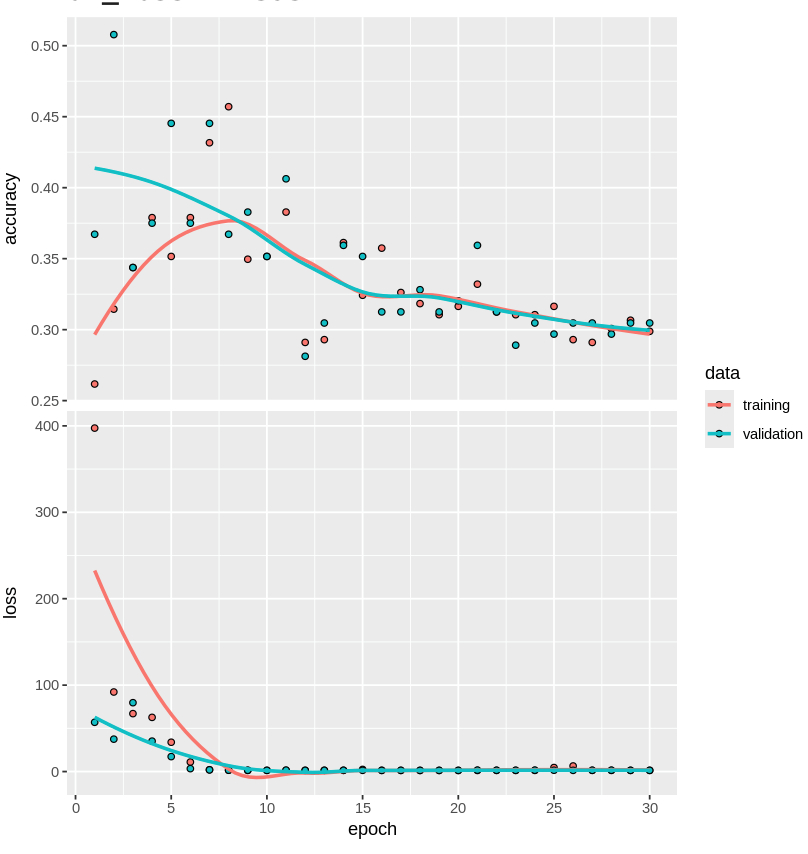
\includegraphics[width=0.5\textwidth]{Results/D1_m1.jpg}
    \caption{Day1-Model1: Accuracy visualization}
    \label{fig:D1_m1}
\end{figure}

The accuracy is around 0.30 in this model. That is expected as the input shape size is huge and other were only 3 layers. Or this can be due to low amount of images (200) for each category. 

\section{Day 2: Building additional NN models on the complex data}

Model 2 and 3:
In model 2 and 3 I increased the amount of layers with different parameters.
Model 2 and 3 Code:
\begin{verbatim}
# Model 2: Adding Another Dense Layer and Dropout
model2 <- keras_model_sequential() %>% 
  
  # First dense layer with 64 units and ReLU activation
  layer_dense(units = 64, activation = 'relu', input_shape = c(196608)) %>% 
  
  # Dropout layer with 60% dropout rate
  layer_dropout(rate = 0.6) %>% 
  
  # Second dense layer with 32 units and ReLU activation
  layer_dense(units = 32, activation = 'relu') %>%
  
  # Dropout layer with 40% dropout rate
  layer_dropout(rate = 0.4) %>%
  
  # Output layer with 4 units and softmax activation
  layer_dense(units = 4, activation = 'softmax')

# Display the model architecture
summary(model2)

# Model 3: Adjusting Sizes and Dropout Rates
model3 <- keras_model_sequential() %>% 
  
  # First dense layer with 128 units and ReLU activation
  layer_dense(units = 128, activation = 'relu', input_shape = c(196608)) %>% 
  
  # Dropout layer with 50% dropout rate
  layer_dropout(rate = 0.5) %>% 
  
  # Second dense layer with 64 units and ReLU activation
  layer_dense(units = 64, activation = 'relu') %>%
  
  # Dropout layer with 30% dropout rate
  layer_dropout(rate = 0.3) %>%
  
  # Output layer with 4 units and softmax activation
  layer_dense(units = 4, activation = 'softmax')

# Display the model architecture
summary(model3)

# Compile both models
model2 %>% compile(
  loss = 'sparse_categorical_crossentropy',
  optimizer = optimizer_rmsprop(),
  metrics = c('accuracy')
)

model3 %>% compile(
  loss = 'sparse_categorical_crossentropy',
  optimizer = optimizer_rmsprop(),
  metrics = c('accuracy')
)

history2 <- model2 %>% fit(
  x_train, y_train, 
  epochs = 30, batch_size = 128, 
  validation_split = 0.2
)
history3 <- model3 %>% fit(
  x_train, y_train, 
  epochs = 30, batch_size = 128, 
  validation_split = 0.2
)
\end{verbatim}
Model 2 evaluation table:
\begin{table}[h!]
    \centering
    \begin{tabular}{|c|c|c|}
        \hline
        \textbf{Metric} & \textbf{Value (Train)} & \textbf{Value (Validation)} \\ \hline
        Accuracy & 0.2637 & 0.2422 \\ \hline
        Loss & 1.38 & 1.376 \\ \hline
    \end{tabular}
    \caption{Day2-Model2: Final Epoch Metrics: Training and Validation}
    \label{tab:D2M2_final_epoch}
\end{table}

Model 3 evaluation table:
\begin{table}[h!]
    \centering
    \begin{tabular}{|c|c|c|}
        \hline
        \textbf{Metric} & \textbf{Value (Train)} & \textbf{Value (Validation)} \\ \hline
        Accuracy & 0.2578 & 0.2734 \\ \hline
        Loss & 1.361 & 1.395 \\ \hline
    \end{tabular}
    \caption{Day2-Model3: Final Epoch Metrics: Training and Validation}
    \label{tab:D2M3_final_epoch}
\end{table}


Model 2 accuracy visualization:
\begin{figure}[H]
    \centering
    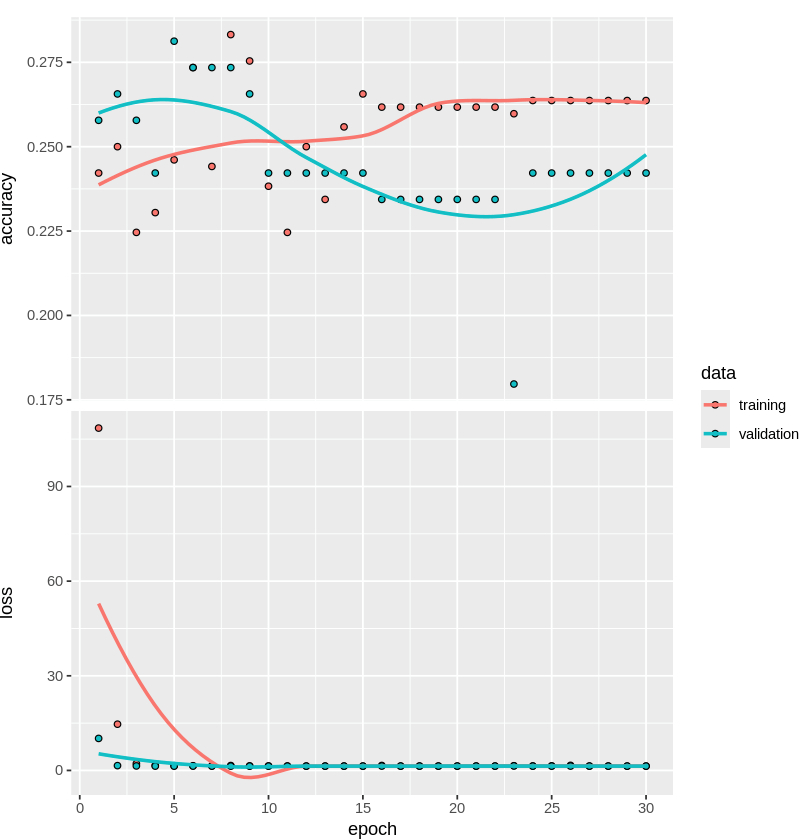
\includegraphics[width=0.5\textwidth]{Results/D2M2.jpg}
    \caption{Day2-Model2: Accuracy visualization}
    \label{fig:D1_m2}
\end{figure}
Model 3 accuracy visualization:
\begin{figure}[H]
    \centering
    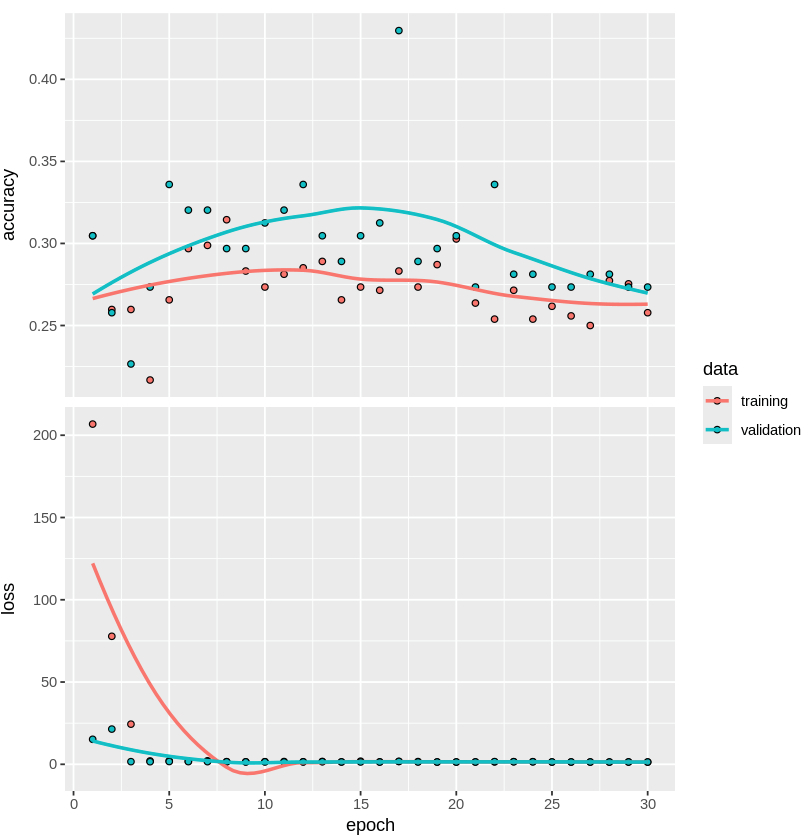
\includegraphics[width=0.5\textwidth]{Results/D2M3.jpg}
    \caption{Day2-Model3: Accuracy visualization}
    \label{fig:D1_m3}
\end{figure}

So, even after increasing the dense layers the accuracy was horrible which is around 0.30 for these three models that were tried in this dataset. Here, I did not build the function to look at the misclassification as all of the models are equally bad.  But it gets better in Day3 when we applied CNN. I used the misclassification function to inspect some of the misclassifications there.

\section{Day 3: Applying CNN and different optimizers}
3 different CNN Model on the MRI data:
\begin{verbatim}
    # Model 1: Convolutional Neural Network with Dropout Layers
model1 <- keras_model_sequential() %>%
  layer_conv_2d(filters = 16, kernel_size = c(3, 3), padding = "same",
                input_shape = c(img_height, img_width, num_channels), activation = "relu") %>%
  layer_max_pooling_2d(pool_size = c(4, 4)) %>%
  layer_dropout(rate = 0.4) %>%
  layer_conv_2d(filters = 32, kernel_size = c(3, 3), padding = "same",
                activation = "relu") %>%
  layer_max_pooling_2d(pool_size = c(2, 2)) %>%
  layer_dropout(rate = 0.8) %>%
  layer_conv_2d(filters = 16, kernel_size = c(3, 3), padding = "same",
                activation = "relu") %>%
  layer_max_pooling_2d(pool_size = c(2, 2)) %>%
  layer_dropout(rate = 0.2) %>%
  layer_flatten() %>%
  layer_dense(units = 64, activation = "relu") %>%
  layer_dense(units = 4, activation = "softmax")

# Display the model architecture
summary(model1)

# Compile the model
model1 %>% compile(
  loss = 'sparse_categorical_crossentropy',
  optimizer = optimizer_rmsprop(),
  metrics = c('accuracy')
)

# Train the Model

history1 <- model1 %>% fit(
  x_train, y_train,
  epochs = 30, batch_size = 32,
  validation_split = 0.2
)

# View training history
history1
plot(history1)

# Build Alternative Models

# Model 2: Adjusted Dropout Rates
model2 <- keras_model_sequential() %>%
  layer_conv_2d(filters = 16, kernel_size = c(3, 3), padding = "same",
                input_shape = c(img_height, img_width, num_channels), activation = "relu") %>%
  layer_max_pooling_2d(pool_size = c(4, 4)) %>%
  layer_dropout(rate = 0.8) %>%
  layer_conv_2d(filters = 32, kernel_size = c(3, 3), padding = "same",
                activation = "relu") %>%
  layer_max_pooling_2d(pool_size = c(2, 2)) %>%
  layer_dropout(rate = 0.8) %>%
  layer_conv_2d(filters = 16, kernel_size = c(3, 3), padding = "same",
                activation = "relu") %>%
  layer_max_pooling_2d(pool_size = c(2, 2)) %>%
  layer_dropout(rate = 0.2) %>%
  layer_flatten() %>%
  layer_dense(units = 64, activation = "relu") %>%
  layer_dense(units = 4, activation = "softmax")

# Display the model architecture
summary(model2)

# Compile the model
model2 %>% compile(
  loss = 'sparse_categorical_crossentropy',
  optimizer = optimizer_rmsprop(),
  metrics = c('accuracy')
)

# Train Model 2
history2 <- model2 %>% fit(
  x_train, y_train,
  epochs = 30, batch_size = 32,
  validation_split = 0.2
)

# Model 3: Simplified Model with Fewer Layers
model3 <- keras_model_sequential() %>%
  layer_conv_2d(filters = 16, kernel_size = c(3, 3), padding = "same",
                input_shape = c(img_height, img_width, num_channels), activation = "relu") %>%
  layer_max_pooling_2d(pool_size = c(4, 4)) %>%
  layer_dropout(rate = 0.8) %>%
  layer_conv_2d(filters = 16, kernel_size = c(3, 3), padding = "same",
                activation = "relu") %>%
  layer_max_pooling_2d(pool_size = c(2, 2)) %>%
  layer_dropout(rate = 0.2) %>%
  layer_flatten() %>%
  layer_dense(units = 64, activation = "relu") %>%
  layer_dense(units = 4, activation = "softmax")

# Display the model architecture
summary(model3)

# Compile the model
model3 %>% compile(
  loss = 'sparse_categorical_crossentropy',
  optimizer = optimizer_rmsprop(),
  metrics = c('accuracy')
)

# Train Model 3
history3 <- model3 %>% fit(
  x_train, y_train,
  epochs = 30, batch_size = 32,
  validation_split = 0.2
)
\end{verbatim}

CNN Model evaluation table:

\begin{table}[h!]
    \centering
    \begin{tabular}{|c|c|c|c|c|}
        \hline
        \textbf{Model} & \textbf{Accuracy (Train)} & \textbf{Loss (Train)} & \textbf{Accuracy (Validation)} & \textbf{Loss (Validation)} \\ \hline
        CNN Model 1 & 0.9082 & 0.2493 & 0.7891 & 0.57 \\ \hline
        CNN Model 2 & 0.9102 & 0.2693 & 0.7891 & 0.6919 \\ \hline
        CNN Model 3 & 0.9883 & 0.04876 & 0.7266 & 1.445 \\ \hline
    \end{tabular}
    \caption{Day 3: Final Epoch Metrics for CNN Models}
    \label{tab:cnn_models}
\end{table}

CNN model accuracy visualization:
\begin{figure}[H]
    \centering
    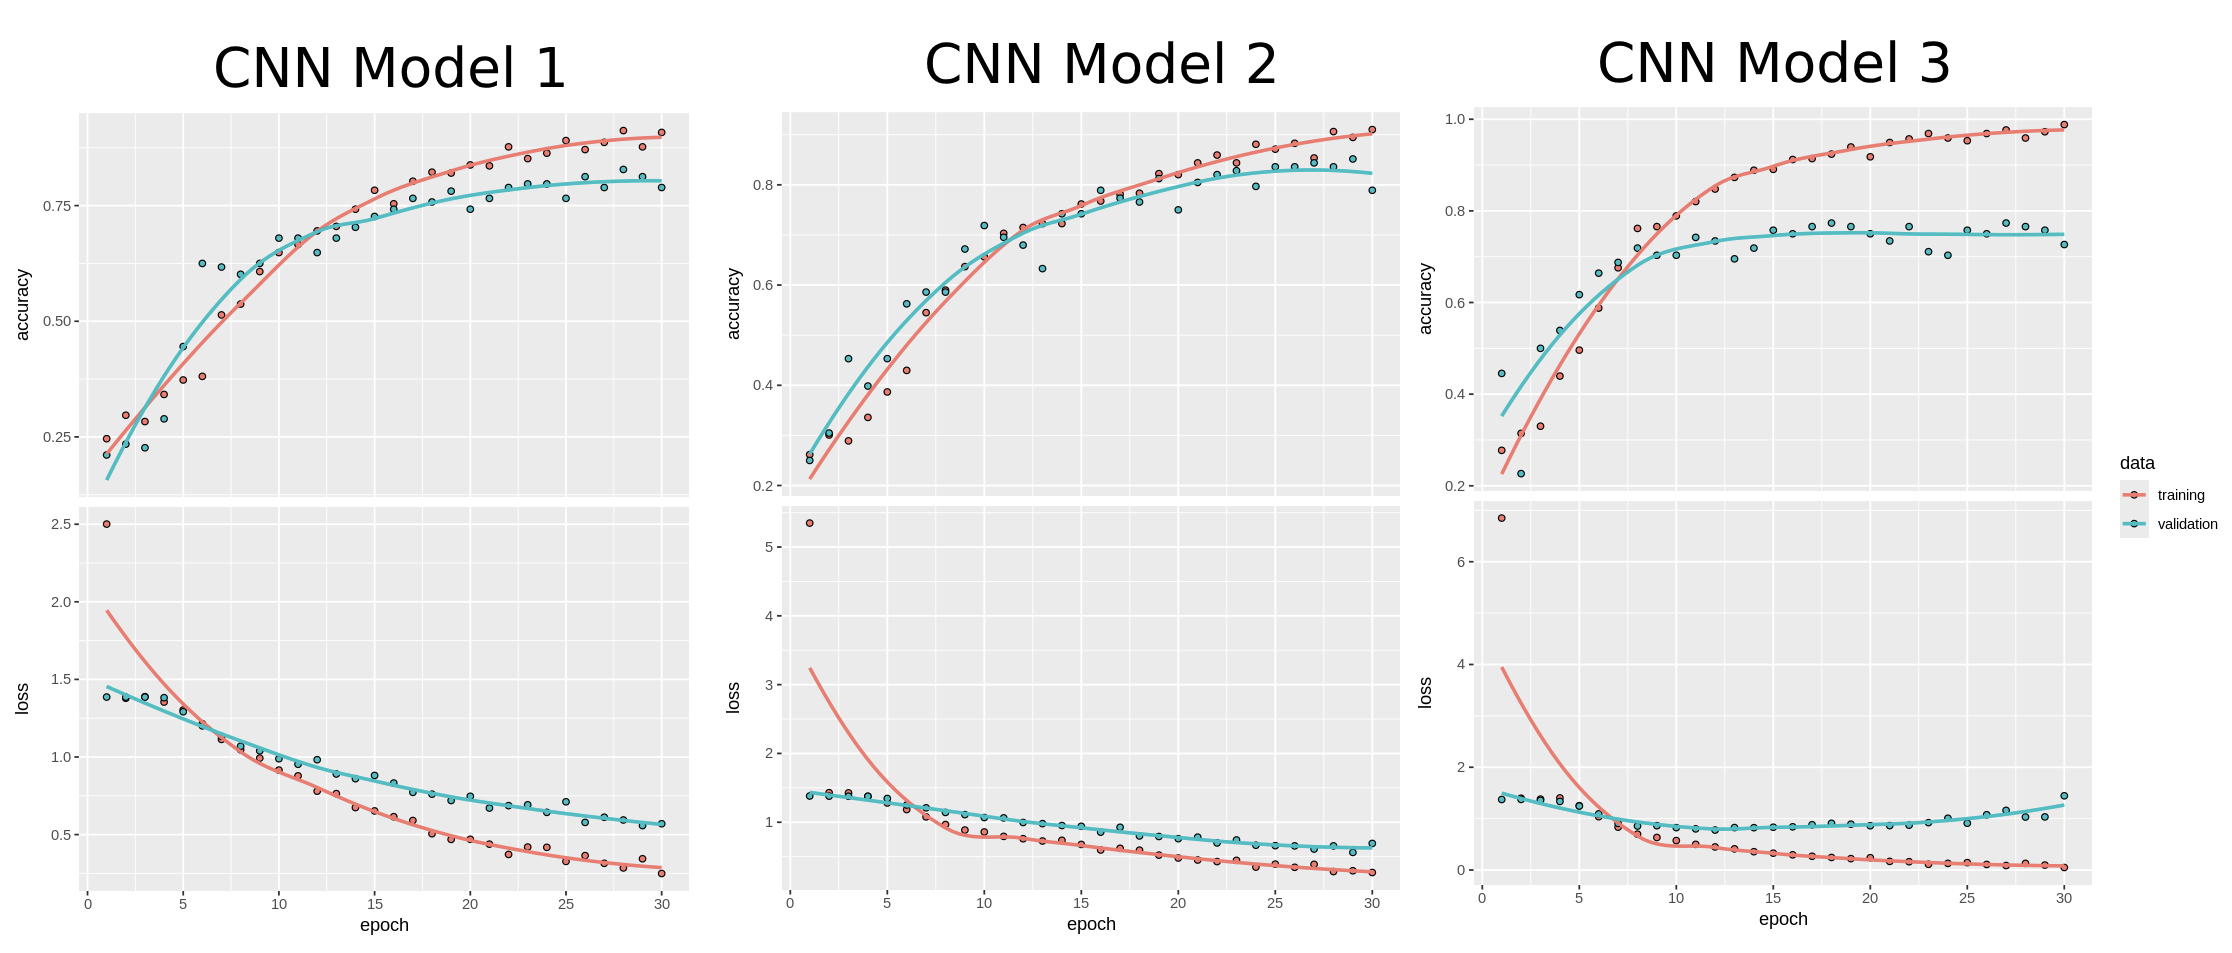
\includegraphics[width=1\textwidth]{Results/CNN models.jpg}
    \caption{Day3-CNN Models and their Accuracy}
    \label{fig:D3_cnn_models}
\end{figure}

After using the CNN models on the same 200 MRI images from each category the accuracy increased tremendously. Model 1 and 2 had similar success. Model 3 accuracy rate was super high but did not do that much well in the validation set. Model 1 and 2 also had some issues with their validation set. Altogether I decided that model 2 might be the best model among these three.

Looking at some misclassified images by CNN model 2:

Model says: meningioma but reality is: normal
\begin{table}[h!]
    \centering
    \begin{tabular}{|c|c|c|}
        \hline
        \textbf{Code} & \textbf{Class} & \textbf{Probability} \\ \hline
        0 & Glioma & 0.007 \\ \hline
        1 & Meningioma & 0.531 \\ \hline
        2 & Normal & 0.434 \\ \hline
        3 & Pituitary & 0.027 \\ \hline
    \end{tabular}
    \caption{Class Probabilities for Different Codes by model 2}
    \label{tab:class_probabilities}
\end{table}

Lets see the misclassified image:
\begin{figure}[H]
    \centering
    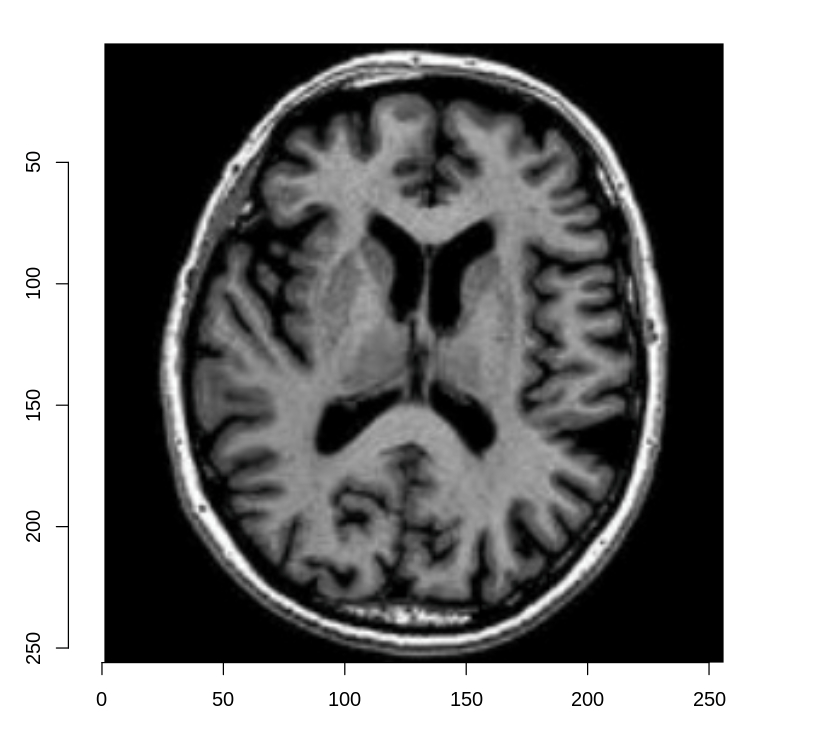
\includegraphics[width=0.3\textwidth]{Results/mri_image.jpg}
    \caption{Day3-CNN Models miss-classification}
    \label{fig:D3_cnn_models}
\end{figure}
Looks like a normal brain image. This can be a model mistake.

Now, I tried 3 different optimizers (optimizer:lamb, optimizer:lion, optimizer:adam) on CNN model 2.

Accuracy evaluation of the three different optimizer:
\begin{table}[h!]
    \centering
    \begin{tabular}{|c|c|c|c|c|}
        \hline
        \textbf{Optimizer} & \textbf{Accuracy (Train)} & \textbf{Loss (Train)} & \textbf{Accuracy (Validation)} & \textbf{Loss (Validation)} \\ \hline
        Lamb & 0.7832 & 0.5524 & 0.7188 & 0.9091 \\ \hline
        Lion & 0.2617 & 1.381 & 0.2344 & 1.409 \\ \hline
        Adam & 0.5703 & 0.9315 & 0.5859 & 1.122 \\ \hline
    \end{tabular}
    \caption{Day 3: Epoch Metrics for Different Optimizers on CNN model 2}
    \label{tab:optimizer_metrics}
\end{table}

None of these optimizer made the CNN model 2 better (made things worst). The original optimizer:rmsprop actually did best.

\section{Day 4: Transfer learning}
Here again, I used 200 images of each tumor category to test whether transfer learning improves my previous models.

Scratch CNN model code:
\begin{verbatim}
    # Define the Convolutional Neural Network model
cnn_model <- keras_model_sequential() %>%
  # First convolutional layer
  layer_conv_2d(filters = 16, kernel_size = c(3, 3), padding = "same", 
                input_shape = c(img_height, img_width, num_channels), activation = "relu") %>%
  layer_max_pooling_2d(pool_size = c(4, 4)) %>%
  layer_dropout(rate = 0.4) %>%
  # Second convolutional layer
  layer_conv_2d(filters = 32, kernel_size = c(3, 3), padding = "same", activation = "relu") %>%
  layer_max_pooling_2d(pool_size = c(2, 2)) %>%
  layer_dropout(rate = 0.3) %>%
  # Third convolutional layer
  layer_conv_2d(filters = 32, kernel_size = c(3, 3), padding = "same", activation = "relu") %>%
  layer_max_pooling_2d(pool_size = c(2, 2)) %>%
  layer_dropout(rate = 0.2) %>%
  # Flatten the output and add dense layers
  layer_flatten() %>%
  layer_dense(units = 64, activation = "relu") %>%
  # Output layer
  layer_dense(units = 4, activation = "softmax")

# Display the model architecture
summary(cnn_model)  

# Compile the CNN model
cnn_model %>% compile(
  loss = 'sparse_categorical_crossentropy',
  optimizer = optimizer_adam(),
  metrics = c('accuracy')
)

# Train the CNN Model -----------------------------------------------------------

cnn_history <- cnn_model %>% fit(
  x_train, y_train,
  batch_size = 32,
  epochs = 10, 
  validation_split = 0.2
)
\end{verbatim}

Transfer learning model:

\begin{verbatim}
    # Load the pre-trained Xception model without the top layers
base_model <- application_xception(
  weights = "imagenet",    # Load weights pre-trained on ImageNet
  include_top = FALSE,     # Do not include the final output layer
  input_shape = c(img_height, img_width, num_channels)  # Adjust input shape
)

# Freeze the base model layers to prevent them from being updated during training
base_model$trainable <- FALSE

# Display the base model architecture
summary(base_model)

# Build the new model on top of the base model
transfer_model <- keras_model_sequential() %>%
  base_model %>%
  # Add global average pooling layer
  layer_global_average_pooling_2d() %>%
  # Add dropout for regularization
  layer_dropout(rate = 0.2) %>%
  # Add output layer
  layer_dense(units = 4, activation = "softmax")

# Display the new model architecture
summary(transfer_model)

# Compile the Transfer Learning Model -------------------------------------------

transfer_model %>% compile(
  loss = 'sparse_categorical_crossentropy',
  optimizer = optimizer_adam(),
  metrics = c('accuracy')
)

# Train the Transfer Learning Model ---------------------------------------------

transfer_history <- transfer_model %>% fit(
  x_train, y_train,
  batch_size = 32,
  epochs = 6, 
  validation_split = 0.2
)
\end{verbatim}

Accuracy evaluation of the scratch CNN model and transfer learning model:

\begin{table}[h!]
    \centering
    \begin{tabular}{|c|c|c|c|c|}
        \hline
        \textbf{Model} & \textbf{Accuracy (Train)} & \textbf{Loss (Train)} & \textbf{Accuracy (Validation)} & \textbf{Loss (Validation)} \\ \hline
        Scratch CNN & 0.8496 & 0.4384 & 0.7812 & 0.6696 \\ \hline
        Transfer Learning & 0.9375 & 0.23 & 0.8359 & 0.4216 \\ \hline
    \end{tabular}
    \caption{Day 4: Final Epoch Metrics: Scratch CNN vs. Transfer Learning Model}
    \label{tab:cnn_transfer}
\end{table}

\begin{figure}[H]
    \centering
    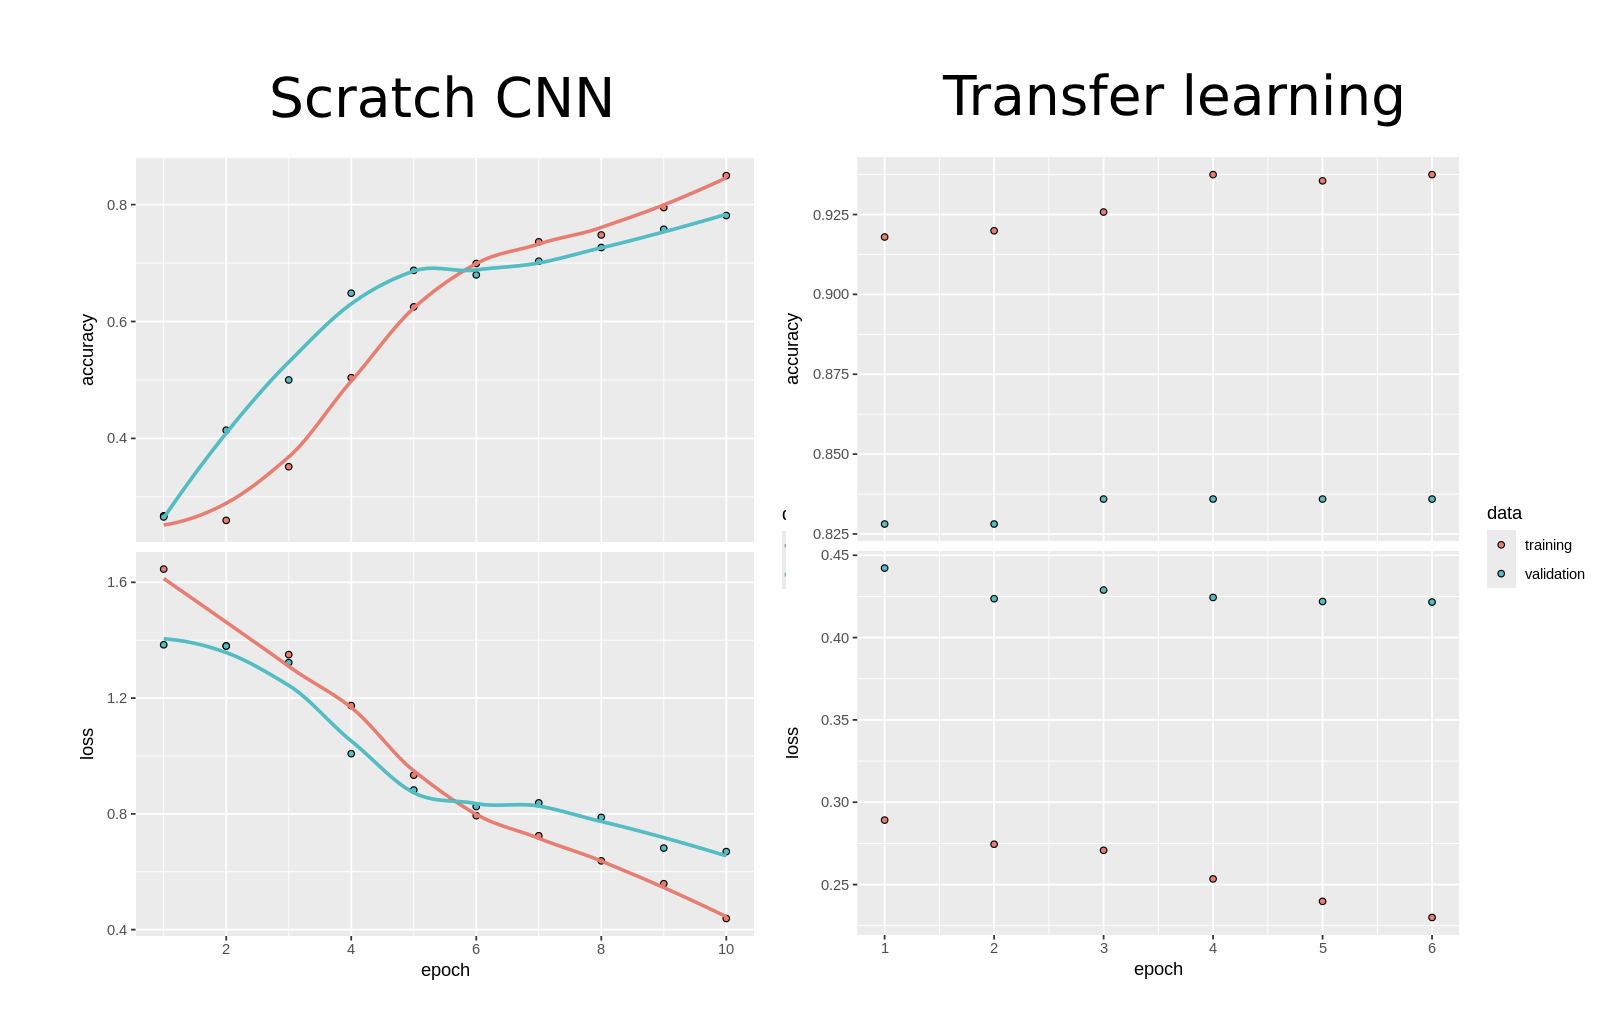
\includegraphics[width=0.8\textwidth]{Results/transfer_learning.jpg}
    \caption{Day 4: Scratch Models and transfer learning evaluation}
    \label{fig:D4_transfer_learning}
\end{figure}

So, the transfer learning improved the scratch CNN. Although the plot of transfer learning looks weird. But if you look at the y-axis scale is between 0.82 to 0.93. It may be over fitted but may be still better than scratch CNN.  


%\bibliographystyle{plain}
%\bibliography{references}

\end{document}